\todo{Write exciting new results in FTS along with questions left to verify.}
\section{Introduction}
Using a control contact draped over \ac{hBN} we demonstrated strong evidence for a normal mode on that exists purely on the hinge or side of the \ac{FTS} crystal\cite{Gray2019}. Recent works have called into question the exact topological nature of \ac{FTS} claiming the crystal is not a topological insulator but rather a topological semi-metal with buried Dirac nodes. In light of this it is crucial to obtain evidence with experimental techniques other than . In this work, we probe much deeper into the characteristics of this mode to better understand the underlying topology of \ac{FTS}. To accomplish this, we investigate the effect the edge quality has on the topological characteristics of \ac{FTS} as it has been previously shown that the quality of the edge of the crystal can have a drastic effect on its transport characteristics \todo{cite Andrea's work on different transport characteristics of graphene}. 

\section{Observation of Bias-Independent Conductance Plateau}
The most striking feature of the resultant $\frac{dI}{dV}$ vs $v_{bias}$ is the bias-independent conductance plateau shown in Fig \ref{fig:PARDeviceFab}. The plateau is exactly twice the value of the high-bias conductance, Simply put, this plateau feature is extremely strong evidence that \ac{PAR} is occurring at the normal-metal/superconductor interface. 
\begin{figure}
    \centering
    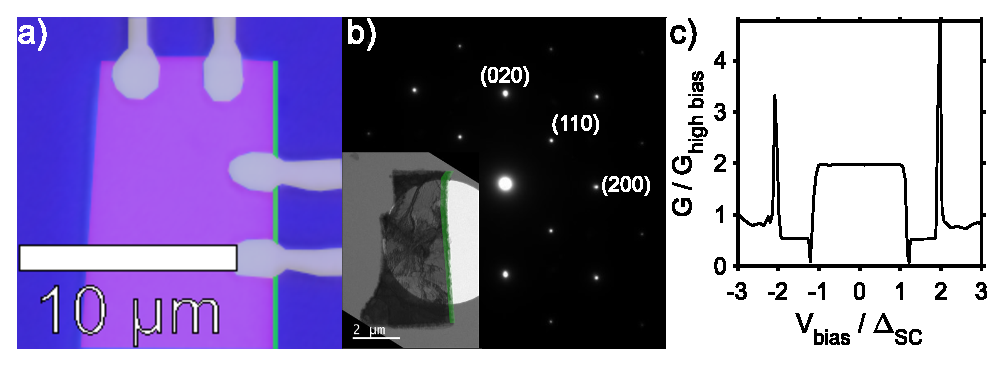
\includegraphics[width = \textwidth]{Chap4/Figures/DeviceFab.eps}
    \caption{a) False color optical image of a representative device with a straight (100) edge. b) \ac{TEM} diffraction pattern demonstrating the (100) edge. Inset shows the flake measured as well as the diffraction aperture. c) Base temperature differential conductance curve.}
    \label{fig:PARDeviceFab}
\end{figure}
\begin{figure}
    \centering
    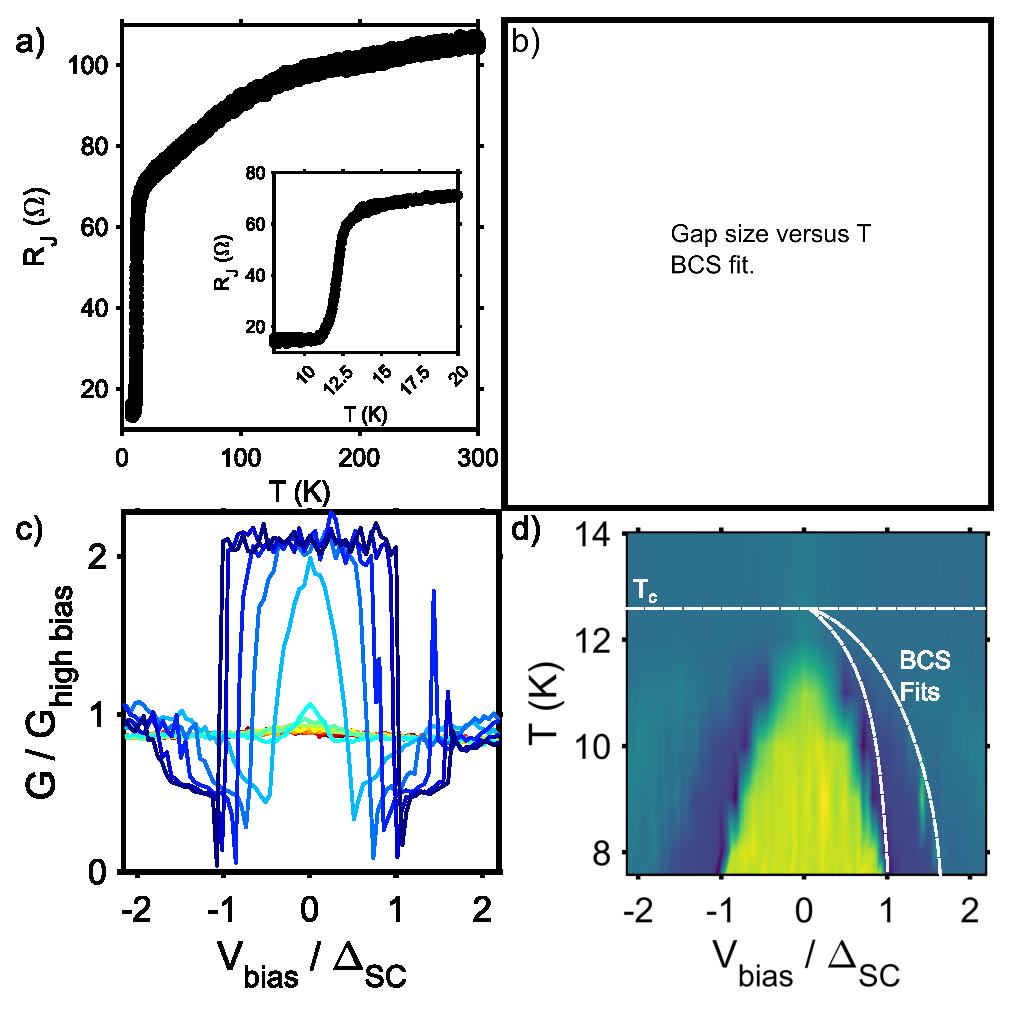
\includegraphics[width = \textwidth]{Chap4/Figures/Temperature.eps}
    \caption{Caption}
    \label{fig:PARTemp}
\end{figure}
\section{Magnetic Field Dependence}
\begin{figure}
    \centering
    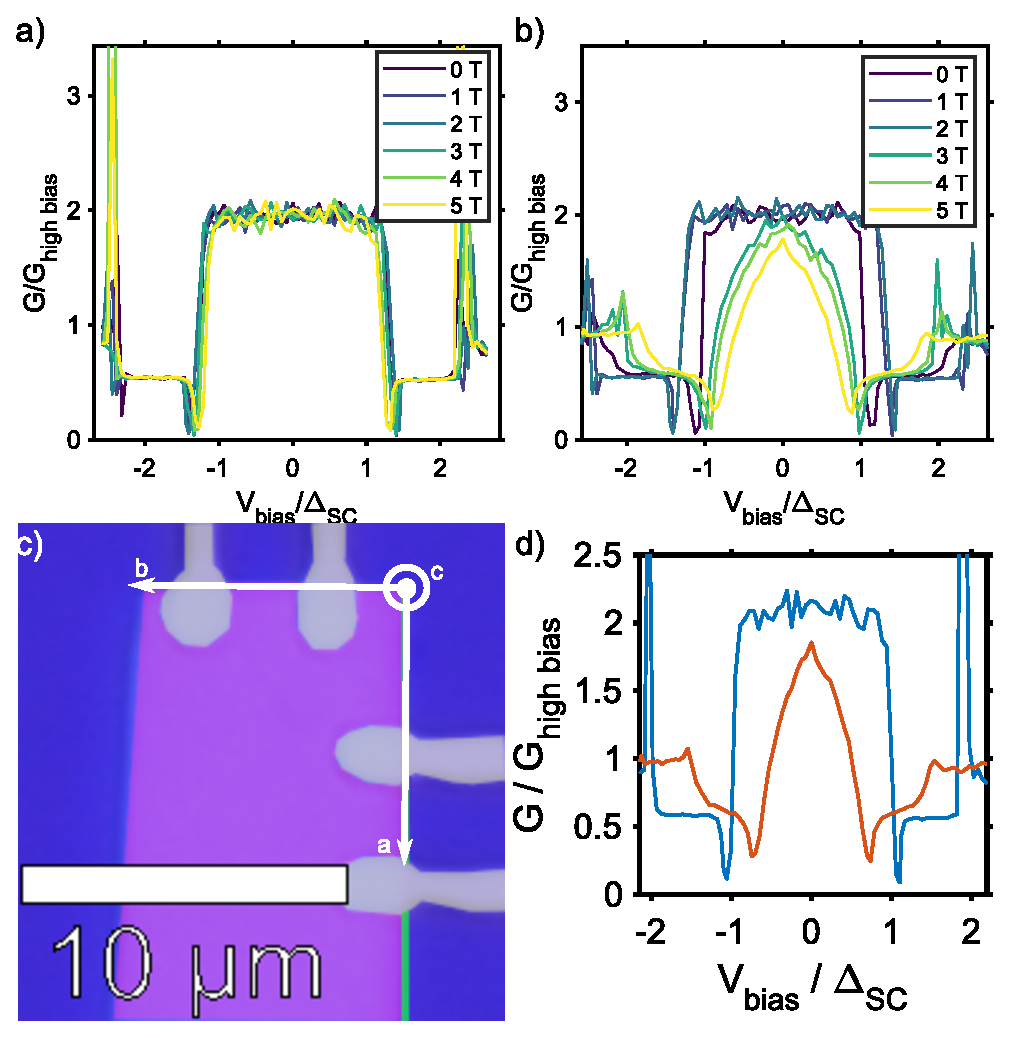
\includegraphics[width = \textwidth]{Chap4/Figures/MagneticField.eps}
    \caption{Caption}
    \label{fig:PARField}
\end{figure}
\section{Conclusion}